\documentclass{beamer}
\usepackage{empheq}
\usepackage[pscoord]{eso-pic}% The zero point of the coordinate systemis the lower left corner of the page (the default).

\usepackage[absolute,overlay]{textpos}
\usepackage[dvipsnames]{xcolor}

\usepackage[ngerman]{babel}

\usepackage{tikz}
\usepackage{biblatex} \usepackage{amsmath} \usepackage{braket} \usepackage{amssymb}
\usepackage[output-decimal-marker={,}]{siunitx}

\usetikzlibrary{arrows.meta, positioning, shapes.geometric, decorations.markings, bending}



%Graphics and Videos
\usepackage{graphicx} %The mode "LaTeX => PDF" allows the following formats: .jpg  .png  .pdf  .mps
\graphicspath{{./images/}} %Where the figures folder is located
\usepackage{media9}
\addmediapath{./videos/}

\addbibresource{refs.bib}

\usetheme{Boadilla}
\title{Bestimmung des Quark-Antiquark Potentials in der Hamiltonschen Formulierung der kompakten U(1) Eichtheorie}
\author{Angelo Valentino Brade} %\institute{Rhenish Friedrich Wilhelm University of Bonn} \institute{University of Bonn} \date{\today}


\makeatother
\setbeamertemplate{footline}
{
  \leavevmode%
  \hbox{%
  \begin{beamercolorbox}[wd=.2\paperwidth,ht=2.25ex,dp=1ex,center]{author in head/foot}%
    \usebeamerfont{author in head/foot}\insertshortauthor
  \end{beamercolorbox}%
  \begin{beamercolorbox}[wd=.4\paperwidth,ht=2.25ex,dp=1ex,center]{section in head/foot}%
    \usebeamerfont{section in head/foot}\insertsectionhead
  \end{beamercolorbox}%
  \begin{beamercolorbox}[wd=.4\paperwidth,ht=2.25ex,dp=1ex,center]{title in head/foot}%
    \usebeamerfont{title in head/foot}\insertshorttitle\hspace*{1em}
    \insertframenumber{} / \inserttotalframenumber\hspace*{1ex}
  \end{beamercolorbox}}%
  \vskip0pt%
}
\makeatletter
\setbeamertemplate{navigation symbols}{}



\begin{document}
\begin{frame}
	\titlepage
\end{frame}
\section{Einleitung}
\begin{frame}
	\frametitle{Übersicht}
	\begin{figure}[h]
		\center\begin{tikzpicture}
	\tikzstyle{box} = [rectangle, minimum width = 2cm, minimum height = 1cm, text centered, draw=black]
	\tikzstyle{tbox} = [rectangle, minimum width = 1cm, minimum height = 0.7cm, text centered, draw=black]
	\tikzstyle{arrow}  = [thick, ->, >=stealth]

	\node[box, fill=green!10](theorie){Theorie};

	\node[box, fill=blue!10, right of=theorie, xshift=3cm](simulation){Simulation};
	\draw[arrow] (theorie) to (simulation);

	\node[box, fill=yellow!10, right of=simulation, xshift=3cm](vorhersage){Vorhersage};
	\draw[arrow] (simulation) to (vorhersage);

	\node[tbox, rounded corners, below of=vorhersage, yshift=-1cm, xshift=0.5cm, text width=2cm](konstanten){Konstanten-\\
		abhängig};
	\draw[arrow] (konstanten) to (vorhersage);

	\node[right of=simulation, xshift=1cm](a0){};
	\node[tbox, rounded corners, below of=a0, yshift=-1cm, xshift=-0.5cm, text width=2cm](eichung){an realen Werten kallibrieren};
	\draw[arrow] (eichung) to (a0);

	\node[left of=konstanten, xshift=-0.5cm]{\large{$\Leftarrow$}};

  \node[right of=theorie, yshift=-0.8cm, xshift=0.2cm](a1){};
  \node[right of=vorhersage, yshift=-0.8cm, xshift=0.2cm](a2){};
  \node[right of=vorhersage, yshift=0.8cm, xshift=0.2cm](a3){};
  \node[right of=theorie, yshift=0.8cm, xshift=0.2cm](a4){};
  \node[above of=simulation, yshift=0.2cm, xshift=1cm](t5){Diese Arbeit};

  \draw[thick, dashed] (a1) to (a2);
  \draw[thick, dashed] (a2) to (a3);
  \draw[thick, dashed] (a3) to (a4);
  \draw[thick, dashed] (a4) to (a1);

\end{tikzpicture}

	\end{figure}
\end{frame}

\begin{frame}
	\frametitle{Methoden für die Simulation in der Gitter Eichtheorie}
	\begin{enumerate}
		\item \textit{Markov chain Monte Carlo (MCMC)} im \textit{Lagrange Formalismus}
		\item Diagonalisierung im \textit{Hamilton Formalismus}
	\end{enumerate}
	\begin{itemize}
		\item Lagrange Formalismus wird mehr genutzt
		      \begin{itemize}
			      \item Hat aber das \textit{Sign Problem} für bestimmte Kopplungsregime, in welchem die Varianz nicht mehr abnimmt\\
			            $\Rightarrow$ Hamiltonsche Formulierung ist notwendig
		      \end{itemize}
	\end{itemize}
\end{frame}

\begin{frame}
	\frametitle{Nachteil der Hamiltonschen Formulierung}
	Das Wachstum der Dimension des Hamiltonians ist
	\begin{itemize}
		\item exponentiell mit Gittergröße
		\item polynomiell mit \textit{Trunkierung}
	\end{itemize}
	$\Rightarrow$ sehr schnell sehr Ressourcenaufwendig
\end{frame}

\begin{frame}
	\frametitle{Lösung durch Quantum Computing}
	\begin{itemize}
		\item exponentielle Rechengeschwindigkeit für Berechnungen mit quantenmechanischen Zuständen
		\item Was genau ist aufwendig in der Hamiltonschen Formulierung? Diagonalisierung vom Hamiltonian
	\end{itemize}
	$\Rightarrow$ Variational Quantum Eigensolver (VQE)
	\begin{itemize}
		\item Herstellung von Quantum Devices noch sehr schwierig
		\item Hamiltonsche Formulierung wegen Sign Problem aber immer relevant
	\end{itemize}
\end{frame}

\begin{frame}
	\frametitle{Ziel}
	\begin{enumerate}
		\item Hamiltonsche Formulierung verstehen
		\item durch Trunkierung mit \textit{exact diagonalisation (ED)} die kompakte U(1) Eichtheorie simulieren
		\item an Quark-Antiquark Potential demonstrieren
	\end{enumerate}
\end{frame}

\section{Diskretesierung}
\begin{frame}
	\frametitle{Gitter}
	\begin{columns}
		\begin{column}{0.5\textwidth}
			\large{Kontinuierlich}
			\\[10pt]
			\begin{figure}[h]
				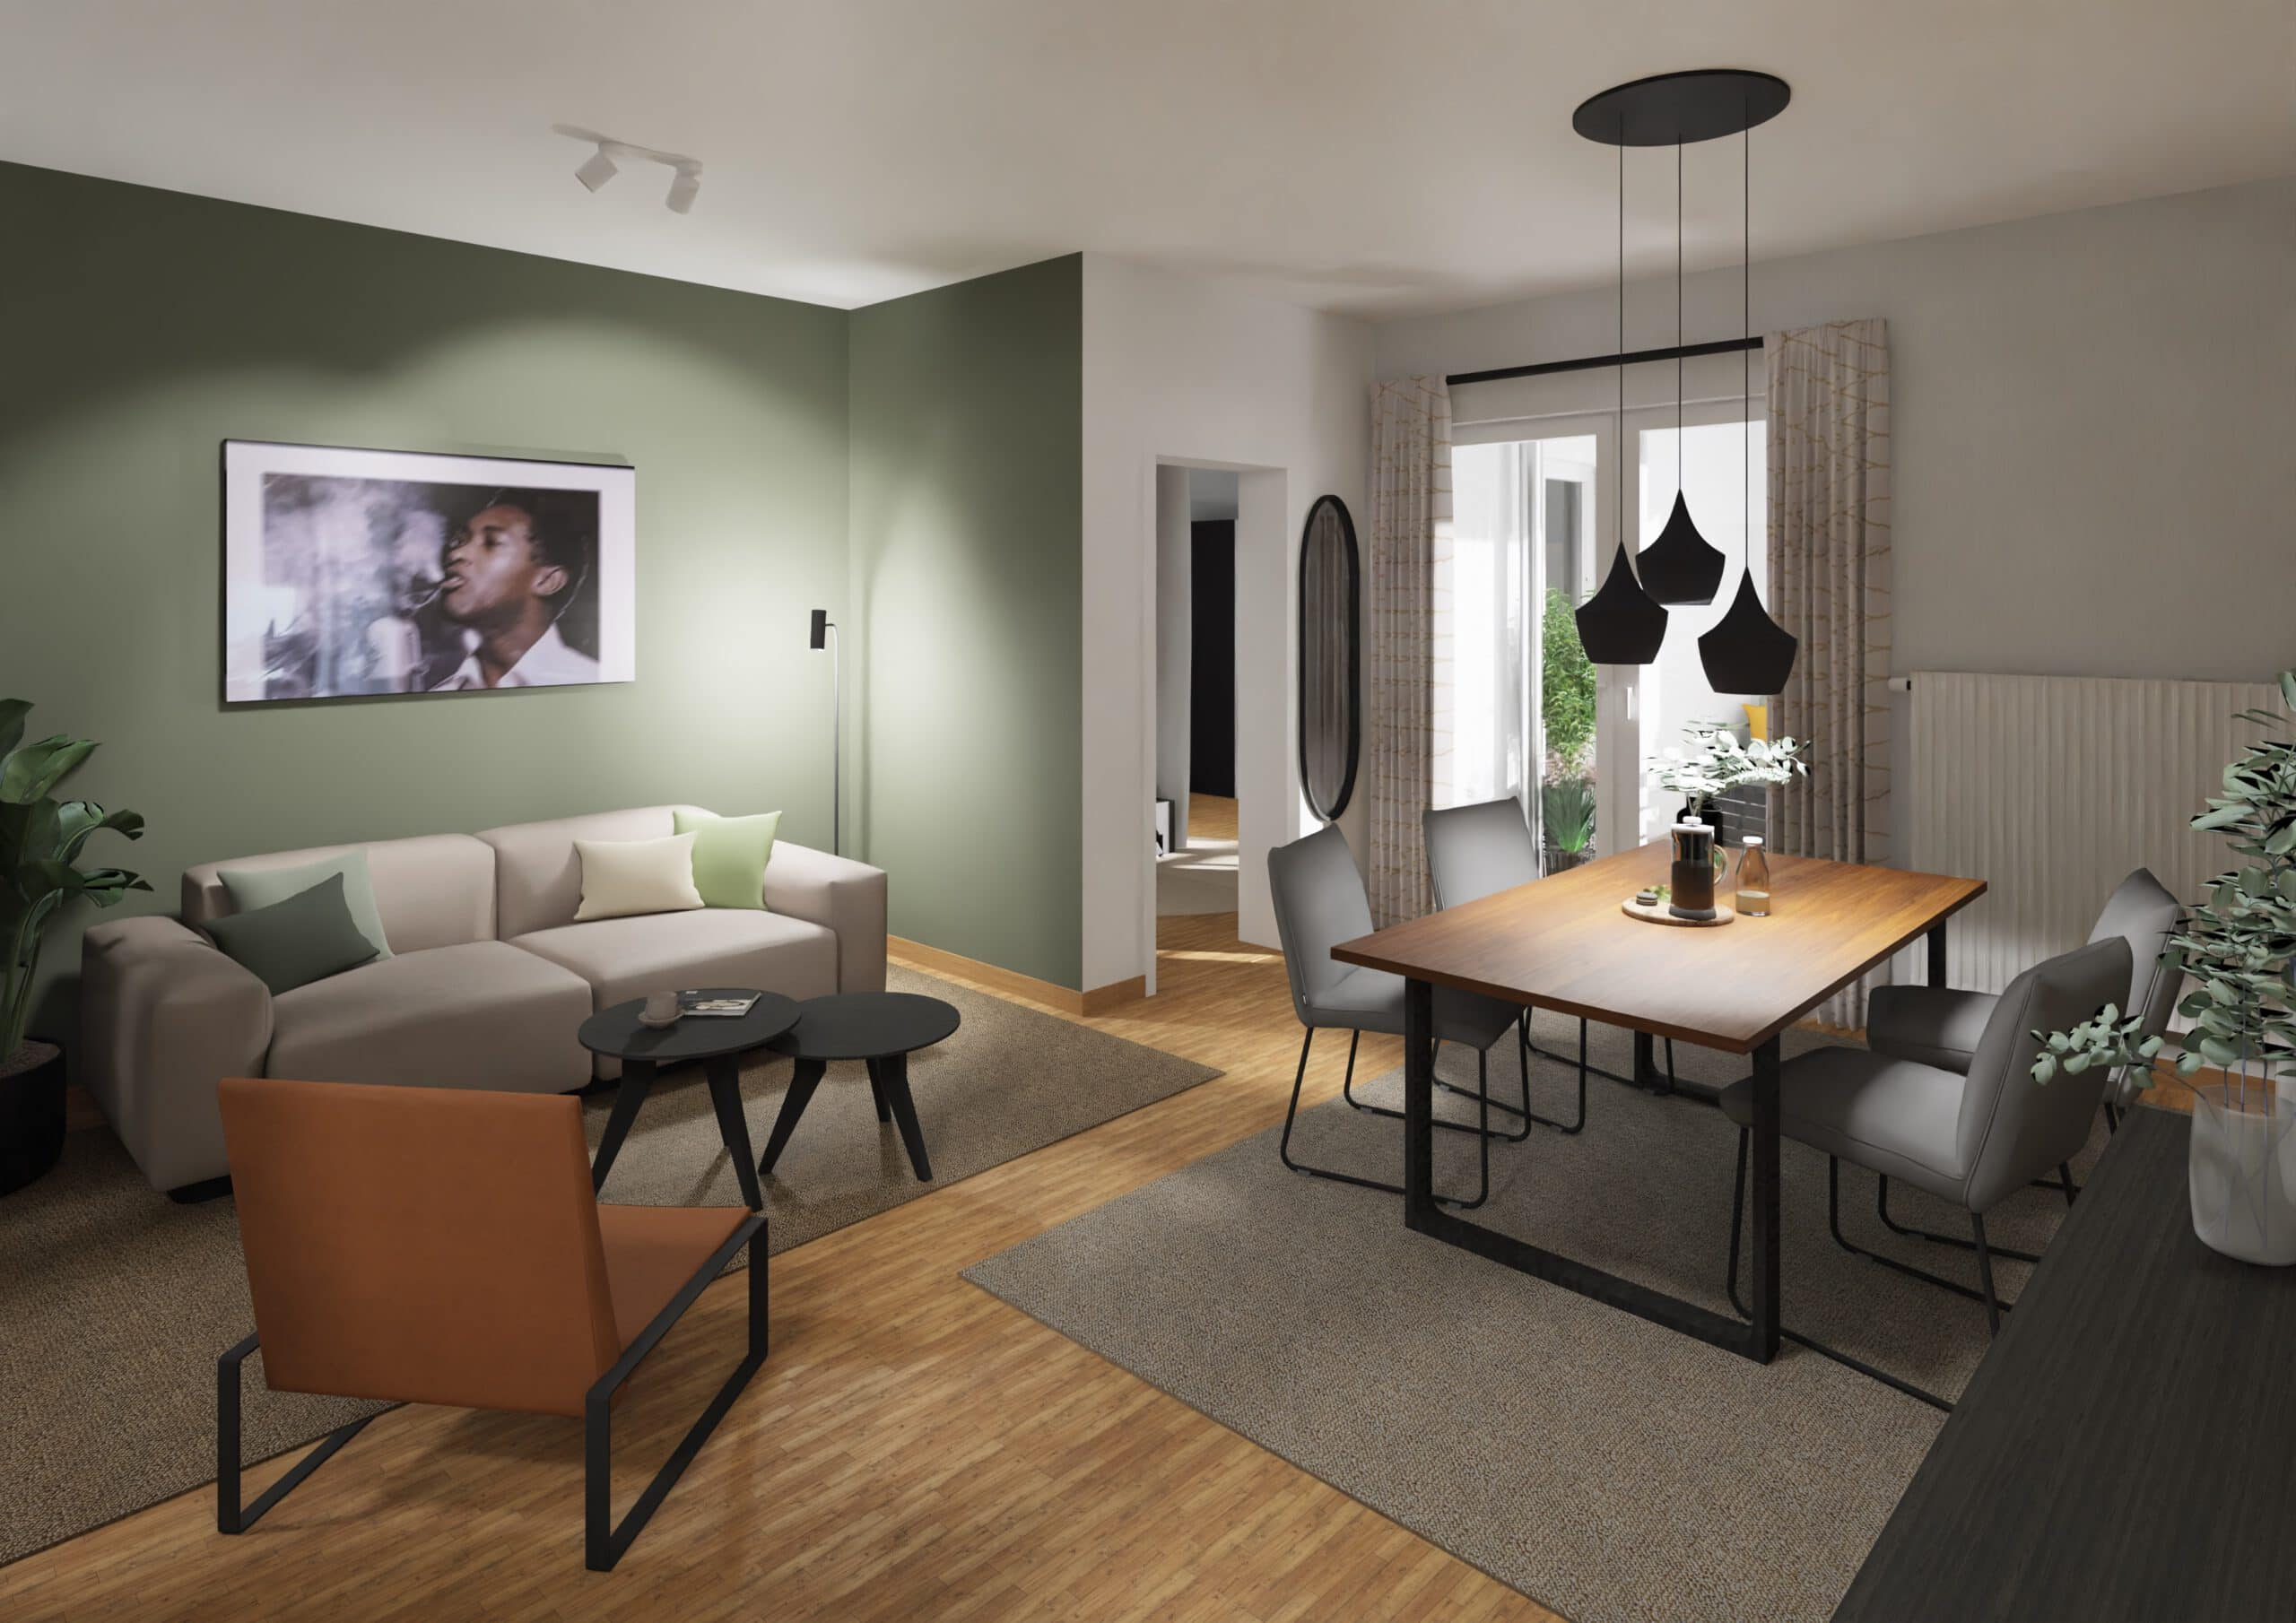
\includegraphics[width=1\textwidth]{Wohnzimmer-1-scaled.jpg}
			\end{figure}
			\tiny{Quelle: Farbmut, 5 Tipps - Räume größer wirken lassen}
		\end{column}
		\begin{column}{0.5\textwidth}
			\large{Diskret}
			\begin{itemize}
				\item Position: $(x, y)\in\mathbb{Z}^{n_x\times n_y}$
				\item Richtung: $\mu\in \{x,y\}$
			\end{itemize}
			\begin{figure}[h]
				\begin{center}
					\begin{tikzpicture}[thick,decoration={
				markings,
				mark=at position 0.5 with {\arrow{>}}}
	]

	\tikzset{
		site/.style={
				circle, draw=gray, fill=gray!20, line width=1.5pt, inner sep=0pt, outer sep=4pt, minimum size=0.4cm
			},
		pcharge/.style={
				circle, draw=red, fill=red!20, line width=1.5pt, inner sep=0pt, outer sep=4pt, minimum size=0.4cm
			},
		ncharge/.style={
				circle, draw=blue, fill=blue!20, line width=1.5pt, inner sep=0pt, outer sep=4pt, minimum size=0.4cm
			},
	}
	\node[site](s1){};
	\node[site, right=0.8cm of s1](s2){};
	\node[site, above=0.8cm of s1](s3){};
  \node[below=1cm of s1, text width=2.5cm](t1){Site: $(x,y)$\\
    trägt Ladung};
	\node[above=0.4cm of s1](a1){};
  \node[left=1cm of s1, text width=2.5cm](t2){Link: ${(x,y),\mu}$\\
    trägt Feld};


	\draw[postaction={decorate}] (s1)--(s2);
	\draw[postaction={decorate}] (s1)--(s3);
  \draw[-{Stealth[length=5mm]}] (t1)--(s1);
  \draw[-{Stealth[length=5mm]}] (t2)--(a1);

\end{tikzpicture}

				\end{center}
			\end{figure}
		\end{column}
	\end{columns}
\end{frame}

\begin{frame}
	\frametitle{$2\times2$ und $3\times3$}
	\begin{figure}[h]
		\begin{center}
			\begin{tikzpicture}[thick,decoration={
				markings,
				mark=at position 0.5 with {\arrow{>}}}
	]

	\tikzset{
		site/.style={
				circle, draw=gray, fill=gray!20, line width=1.5pt, inner sep=0pt, outer sep=4pt, minimum size=0.4cm
			},
		pcharge/.style={
				circle, draw=red, fill=red!20, line width=1.5pt, inner sep=0pt, outer sep=4pt, minimum size=0.4cm
			},
		ncharge/.style={
				circle, draw=blue, fill=blue!20, line width=1.5pt, inner sep=0pt, outer sep=4pt, minimum size=0.4cm
			},
	}
	\node[site](s1){};
	\node[site, right=0.8cm of s1](s2){};
	\node[site, above=0.8cm of s1](s3){};
	\node[site, above=0.8cm of s2](s4){};

	\draw[postaction={decorate}] (s1)--(s2);
	\draw[postaction={decorate}] (s1)--(s3);
	\draw[postaction={decorate}] (s3)--(s4);
	\draw[postaction={decorate}] (s2)--(s4);


  \node[below=0.4cm of s1](a1){};

  \node[above=1cm of s3](a2){};
  \node[right=0cm of a2](t2){\large{$n=2$}};

  
	\node[site, right=4cm of a1](e1){};
	\node[site, right=0.8cm of e1](e2){};
	\node[site, above=0.8cm of e1](e3){};
	\node[site, above=0.8cm of e2](e4){};
	\node[site, right=0.8cm of e2](e5){};
	\node[site, right=0.8cm of e4](e6){};
	\node[site, above=0.8cm of e4](e7){};
	\node[site, above=0.8cm of e3](e8){};
	\node[site, above=0.8cm of e6](e9){};

  \node[above=1cm of e8](a3){};
  \node[right=0.7cm of a3](t2){\large{$n=3$}};

	\draw[postaction={decorate}] (e1)--(e2);
	\draw[postaction={decorate}] (e1)--(e3);
	\draw[postaction={decorate}] (e3)--(e4);
	\draw[postaction={decorate}] (e2)--(e4);
	\draw[postaction={decorate}] (e2)--(e5);
	\draw[postaction={decorate}] (e3)--(e8);
	\draw[postaction={decorate}] (e4)--(e7);
	\draw[postaction={decorate}] (e4)--(e6);
	\draw[postaction={decorate}] (e6)--(e9);
	\draw[postaction={decorate}] (e7)--(e9);
	\draw[postaction={decorate}] (e8)--(e7);
	\draw[postaction={decorate}] (e5)--(e6);

\end{tikzpicture}

		\end{center}
	\end{figure}
\end{frame}

\begin{frame}
	\frametitle{$2\times2$ mit \textit{periodic boundary conditions (PBC)}}
	\begin{figure}[h]
		\begin{center}
			\begin{tikzpicture}[thick,decoration={
				markings,
				mark=at position 0.5 with {\arrow{>}}}
	]

	\tikzset{
		site/.style={
				circle, draw=gray, fill=gray!20, line width=1.5pt, inner sep=0pt, outer sep=4pt, minimum size=0.4cm
			},
		pcharge/.style={
				circle, draw=red, fill=red!20, line width=1.5pt, inner sep=0pt, outer sep=4pt, minimum size=0.4cm
			},
		ncharge/.style={
				circle, draw=blue, fill=blue!20, line width=1.5pt, inner sep=0pt, outer sep=4pt, minimum size=0.4cm
			},
	}
	\node[site](s1){};
	\node[site, right=1.5cm of s1](s2){};
	\node[site, above=1.5cm of s1](s3){};
	\node[site, above=1.5cm of s2](s4){};

	\draw[postaction={decorate}] (s1) to[out=45,in=135] (s2);
	\draw[postaction={decorate}] (s1) to[out=45,in=-45] (s3);
	\draw[postaction={decorate}] (s3) to[out=-45,in=-135] (s4);
	\draw[postaction={decorate}] (s2) to[out=135,in=-135] (s4);

	\draw[postaction={decorate}] (s2) to[out=-135,in=-45] (s1);
	\draw[postaction={decorate}] (s3) to[out=-135,in=135] (s1);
	\draw[postaction={decorate}] (s4) to[out=-45,in=45] (s2);
	\draw[postaction={decorate}] (s4) to[out=135,in=45] (s3);


	\node[site, right=4cm of s1](e1){};
	\node[site, right=1.5cm of e1](e2){};
	\node[site, above=1.5cm of e1](e3){};
	\node[site, above=1.5cm of e2](e4){};
	\node[above=1.5cm of e4](a1){};
	\node[right=1.5cm of e4](a2){};
	\node[right=1.5cm of e2](a3){};
	\node[above=1.5cm of e3](a4){};

  \node[above=0.75cm of s1](a9){};
  \node[right=3.05cm of a9](a8){\huge{$\Leftrightarrow$}};



	\draw[postaction={decorate}] (e1) to (e2);
	\draw[postaction={decorate}] (e1) to (e3);
	\draw[postaction={decorate}] (e3) to (e4);
	\draw[postaction={decorate}] (e2) to (e4);

	\draw[postaction={decorate}] (e2) to (a3);
	\draw[postaction={decorate}] (e3) to (a4);
	\draw[postaction={decorate}] (e4) to (a1);
	\draw[postaction={decorate}] (e4) to (a2);



\end{tikzpicture}

		\end{center}
	\end{figure}
\end{frame}

\section{Hamiltonsche Formulierung}
\begin{frame}
	\frametitle{Ladungen und Felder}
	\begin{columns}
		\begin{column}{0.5\textwidth}
			\begin{itemize}
				\item Ladungen $Q_{\vec{r}}$ und $Q_{\vec{r}+y}$ an Site $\vec{r}$ und $\vec{r} + y$
				\item kanonisch konjugierte Felder $\hat{E}_{\vec{r}, y}$ und $\hat{A}_{\vec{r}, y}$ am Link $\vec{r}, y$
				\item $\vec{r} + y = (r_x, r_y + 1)$
				\item $[\hat{E}_{\vec{r}_j, \mu}, \hat{A}_{\vec{r}_k, \nu}] = i\delta^{(3)}(\vec{r}_j-\vec{r}_k)\delta_{\mu\nu}$
				\item $\hat{E}_{\vec{r}, \mu}\ket{\hat{e}_{\vec{r}, \mu}}=\hat{e}_{\vec{r}, \mu}\ket{\hat{e}_{\vec{r}, \mu}}$
			\end{itemize}
		\end{column}
		\begin{column}{0.5\textwidth}
			\begin{figure}[h]
				\begin{tikzpicture}[thick,decoration={
				markings,
				mark=at position 0.5 with {\arrow{>}}}
	]

	\tikzset{
		site/.style={
				circle, draw=gray, fill=gray!20, line width=1.5pt, inner sep=0pt, outer sep=4pt, minimum size=0.4cm
			},
		pcharge/.style={
				circle, draw=red, fill=red!20, line width=1.5pt, inner sep=0pt, outer sep=4pt, minimum size=0.4cm
			},
		ncharge/.style={
				circle, draw=blue, fill=blue!20, line width=1.5pt, inner sep=0pt, outer sep=4pt, minimum size=0.4cm
			},
	}
	\node[site](s1){};
	\node[site, above of=s1, yshift=1cm](s2){};

	\draw[postaction={decorate}] (s1)--(s2);

  \node[above of=s1, yshift=0.2cm, xshift=-0.9cm](t1){$\hat{E}_{\vec{r}, y}$, $\hat{A}_{\vec{r}, y}$};
  \node[below of=s1, yshift=0.4cm](t2){$Q_{\vec{r}}$};
  \node[above of=s2, yshift=-0.4cm](t2){$Q_{\vec{r}+y}$};

\end{tikzpicture}

			\end{figure}
		\end{column}
	\end{columns}
\end{frame}
\begin{frame}
	\frametitle{Link Operator}
	\begin{columns}
		\begin{column}{0.6\textwidth}
			\begin{itemize}
				\item $\hat{A}_{\vec{r}, \mu}$ generiert aus aus der Lie Algebra $\mathfrak{g}=$u(n) die Lie Gruppe G=U(n)
				\item $\hat{U}_{\vec{r}, \mu}=\exp{(iag\hat{A}_{\vec{r}, \mu})}$ mit $ag\hat{A}_{\vec{r}, \mu}\in[0,2\pi)$ \\
				      $\Rightarrow$ komakte U(1) Theorie
				\item $[\hat{E}_{\vec{r}_{i}, \mu}, \hat{U}_{\vec{r}_{j}, \nu}]      =\delta^{(3)}(\vec{r}_{i}-\vec{r}_{j})\delta_{\mu\nu}\hat{U}_{\vec{r}_{j}, \nu}$
				\item $[\hat{E}_{\vec{r}_{i}, \mu}, \hat{U}_{\vec{r}_{j}, \nu}^\dag] =-\delta^{(3)}(\vec{r}_{i}-\vec{r}_{j})\delta_{\mu\nu}\hat{U}_{\vec{r}_{j}, \nu}^{\dag}.$
				\item $\Rightarrow \hat{U}_{\vec{r}, \mu}\ket{\hat{e}_{\vec{r}, \mu}}=\ket{\hat{e}_{\vec{r}, \mu}-1}$
				\item $\Rightarrow \hat{U^\dag}_{\vec{r}, \mu}\ket{\hat{e}_{\vec{r}, \mu}}=\ket{\hat{e}_{\vec{r}, \mu}+1}$
			\end{itemize}
		\end{column}
		\begin{column}{0.4\textwidth}
		\end{column}

	\end{columns}
\end{frame}

\begin{frame}
	\frametitle{Trunkierung}
	\begin{columns}
		\begin{column}{0.5\textwidth}
			\begin{itemize}
				\item $ag\hat{A}_{\vec{r}, \mu}\in[0,2\pi)$\\
				      $\rightarrow ag\hat{A}_{\vec{r}, \mu}\in[-l,l]$\\
				      mit $[-l,l]=\{-l,-l+1,\dots,l-1,l\}$
				\item $\Rightarrow e_{\vec{r}, \mu} \in [-l,l]$
				\item nurnoch endlich viele Zustände an einem Link möglich: $N_Z=2l+1$
			\end{itemize}
		\end{column}
		\begin{column}{0.5\textwidth}
			$\hat{U}_{\vec{r}, \mu}=\exp{(iag\hat{A}_{\vec{r}, \mu})}$\\
			\,\\
			U(1) $\subset \mathbb{C}, \{\frac{2\pi k}{2l+1}\}_{k\in\mathbb{Z}_{2l+1}}$\\
			\begin{figure}[h]
				\begin{tikzpicture}
  % Draw the main circle (S^1)
\draw[thick] (0,0) circle(1);

% Parameters
\def\n{5}      % Number of truncation lines (Z5)
\def\r{1}      % Radius of the circle
\def\len{0.2}  % Length of the inward lines

% Draw the 5 truncation lines
\foreach \k in {0,...,4} {
  \draw[thick]
    ({\r*cos(360/\n*\k)}, {\r*sin(360/\n*\k)}) % start point on circle
    -- ({(\r-\len)*cos(360/\n*\k)}, {(\r-\len)*sin(360/\n*\k)}); % inward point
}

\node at (1.2, 0) {$0$};
\node at (0, 1.3) {$\frac{\pi}{2}$};
\node at (-1.2, 0) {$\pi$};
\node at (0, -1.3) {$\frac{3\pi}{2}$};

  
\end{tikzpicture}

			\end{figure}
		\end{column}
	\end{columns}
\end{frame}

\begin{frame}
	\frametitle{Hamiltonian}
	\begin{columns}
		\begin{column}{0.5\textwidth}
			\begin{itemize}
				\item $\hat{H}=\frac{g^2}{2}\sum_{\vec{r}}(\hat{E}_{\vec{r}, x}^2+\hat{E}_{\vec{r}, y}^2)-\frac{1}{2a^2g^2}\sum_{\vec{r}}(\hat{P}_{\vec{r}}+\hat{P}_{\vec{r}}^\dag)$\\
				      mit $\hat{P}_{\vec{r}}=\hat{U}_{\vec{r}, x}\hat{U}_{\vec{r}+x,y}\hat{U}^{\dag}_{\vec{r}+y,x}\hat{U}^{\dag}_{\vec{r},y}$
				\item $H_{ij}=\bra{i}\hat{H}\ket{j}$\\
				      mit $\ket{j}\in\mathcal{H}$,\\
              wobei $\ket{j}=\bigotimes_\text{links}\ket{e^{(j)}_{\vec{r}, \mu}}$
			\end{itemize}
		\end{column}
		\begin{column}{0.5\textwidth}
			\begin{figure}
				\begin{tikzpicture}[thick,decoration={
				markings,
				mark=at position 0.5 with {\arrow{>}}}
	]

	\tikzset{
		site/.style={
				circle, draw=gray, fill=gray!20, line width=1.5pt, inner sep=0pt, outer sep=4pt, minimum size=0.4cm
			},
		pcharge/.style={
				circle, draw=red, fill=red!20, line width=1.5pt, inner sep=0pt, outer sep=4pt, minimum size=0.4cm
			},
		ncharge/.style={
				circle, draw=blue, fill=blue!20, line width=1.5pt, inner sep=0pt, outer sep=4pt, minimum size=0.4cm
			},
	}

	\node[site](e1){};
	\node[site, right=1.5cm of e1](e2){};
	\node[site, above=1.5cm of e1](e3){};
	\node[site, above=1.5cm of e2](e4){};
	\node[above=1.5cm of e4](a1){};
	\node[right=1.5cm of e4](a2){};
	\node[right=1.5cm of e2](a3){};
	\node[above=1.5cm of e3](a4){};

  \node[above of=e1, yshift=-0.7cm, xshift=0.3cm] (p11) {};
  \node[above of=e1, yshift=-0.7cm, xshift=1.9cm] (p12) {};
  \node[above of=e1, yshift=0.9cm, xshift=1.9cm] (p13) {};
  \node[above of=e1, yshift=0.9cm, xshift=0.3cm] (p14) {};
  \draw[postaction={decorate}, dashed] (p11) to (p12);
  \draw[postaction={decorate}, dashed] (p12) to (p13);
  \draw[postaction={decorate}, dashed] (p13) to (p14);
  \draw[postaction={decorate}, dashed] (p14) to (p11);
  \node[] at (1.1,1.1) {$\hat{P}_{(0,0)}$};

  \node[above of=e2, yshift=-0.7cm, xshift=0.3cm] (p21) {};
  \node[above of=e2, yshift=-0.7cm, xshift=1.9cm] (p22) {};
  \node[above of=e2, yshift=0.9cm, xshift=1.9cm] (p23) {};
  \node[above of=e2, yshift=0.9cm, xshift=0.3cm] (p24) {};
  \draw[postaction={decorate}, dashed] (p21) to (p22);
  \draw[postaction={decorate}, dashed] (p22) to (p23);
  \draw[postaction={decorate}, dashed] (p23) to (p24);
  \draw[postaction={decorate}, dashed] (p24) to (p21);
  \node[] at (3.3,1.1) {$\hat{P}_{(1,0)}$};

  \node[above of=e3, yshift=-0.7cm, xshift=0.3cm] (p31) {};
  \node[above of=e3, yshift=-0.7cm, xshift=1.9cm] (p32) {};
  \node[above of=e3, yshift=0.9cm, xshift=1.9cm] (p33) {};
  \node[above of=e3, yshift=0.9cm, xshift=0.3cm] (p34) {};
  \draw[postaction={decorate}, dashed] (p31) to (p32);
  \draw[postaction={decorate}, dashed] (p32) to (p33);
  \draw[postaction={decorate}, dashed] (p33) to (p34);
  \draw[postaction={decorate}, dashed] (p34) to (p31);
  \node[] at (1.1,3.3) {$\hat{P}_{(0,1)}$};

  \node[above of=e4, yshift=-0.7cm, xshift=0.3cm] (p41) {};
  \node[above of=e4, yshift=-0.7cm, xshift=1.9cm] (p42) {};
  \node[above of=e4, yshift=0.9cm, xshift=1.9cm] (p43) {};
  \node[above of=e4, yshift=0.9cm, xshift=0.3cm] (p44) {};
  \draw[postaction={decorate}, dashed] (p41) to (p42);
  \draw[postaction={decorate}, dashed] (p42) to (p43);
  \draw[postaction={decorate}, dashed] (p43) to (p44);
  \draw[postaction={decorate}, dashed] (p44) to (p41);
  \node[] at (3.3,3.3) {$\hat{P}_{(1,1)}$};

	\draw[postaction={decorate}] (e1) to (e2);
	\draw[postaction={decorate}](e1) to (e3);
	\draw[postaction={decorate}] (e3) to (e4);
	\draw[postaction={decorate}] (e2) to (e4);

	\draw[postaction={decorate}] (e2) to (a3);
	\draw[postaction={decorate}] (e3) to (a4);
	\draw[postaction={decorate}] (e4) to (a1);
	\draw[postaction={decorate}] (e4) to (a2);
\end{tikzpicture}

			\end{figure}
		\end{column}
	\end{columns}

\end{frame}

\begin{frame}
	\frametitle{Gaußsches Gesetz}
	\begin{itemize}
		\item Nicht alle Gitterzustände aus $\mathcal{H}$ möglich
		\item Nur wenn die Felder sich zu der vorhernaden Ladung aufsummieren, physikalisch möglich $\Rightarrow \oint_A \vec{E} \cdot \text{d}\vec{A}=\frac{Q}{\epsilon_0} \rightarrow \left[\sum_{\mu\in\{x, y\}}(\hat{E}_{\vec{r}, \mu}^2-\hat{E}_{\vec{r}+\mu, \mu}^2)-Q_{\vec{r}}\right]\ket{\Psi}=0$
		\item Felder $\ket{\Psi}$ sind physikalisch:\\
		      $\ket{\Psi}\in\mathcal{H}_\text{phys}\subset\mathcal{H}$
		\item Gaußsches Gesetz gilt an allen $N_S$ Gitterpunkten $\Rightarrow$ wir haben ein LGS aus $N_S$ Gleichungen
		\item LGS ist unterbestimmt und kann nach E-Feldern aufgelöst werden, die frei wählbar sind und \textit{dynamic links} genannte werden
		\item $\Rightarrow \hat{E}_{\vec{r}, \text{fixed}}$ sind Linearkombination aus dynamischen links
		\item $\Rightarrow \hat{U}_{\vec{r}, \text{fixed}}$ müsse in den Plaquettes nicht mehr beachtet werden, da sie automatisch unphysikalische Gitterzustände erzeugen
	\end{itemize}
\end{frame}
\begin{frame}
	\frametitle{Beispiel: $2\times2$}
	\begin{itemize}
		\item Gaußsche Gesetze\\
		      $E_{(0, 0), x}+E_{(0,0), y}=0$, $E_{(0, 1), y}-E_{(0, 0), x}=0$,\\
		      $-E_{(0, 1), y}-E_{(1, 0), x}=0$ und $E_{(1, 0), x}-E_{(0,0), y}=0$\\
		      $\Rightarrow E_{(0, 0), y}=-E_{(0, 0), x}, E_{(0, 1), y}=E_{(0, 0), x}, E_{(1, 0), x}=-E_{(0, 0), x}$\\
		      $\Rightarrow \hat{E}_{(0, 0), x}$ ist dynamisch und nur $\hat{U}_{(0, 0), x}$ kann wirken
		\item Trunkierung: $l=1$ $\Rightarrow 2l+1=3$\\
		      $\Rightarrow$ Zustände $\ket{-1}, \ket{0}$ und $\ket{1}$ möglich
		\item $H_{ij}=\bra{i}\hat{H}\ket{j}$ mit $a=1$ und $g=1$:\\
		      $ \hat{H}=
			      \begin{pmatrix}
				      2           & \frac{1}{2} & 0           \\
				      \frac{1}{2} & 0           & \frac{1}{2} \\
				      0           & \frac{1}{2} & 2
			      \end{pmatrix}
			      \Rightarrow E_0=\num{2}$, $E_1\approx-\num{0.22}$, $E_2\approx\num{2.22}
		      $
        \item Da $E_1$ den kleinsten Wert hat, ist der Eigenvektor zu $E_1$ der Grundzustand des Gitters
  \item Können wir jedes Gitter einfach auf Papier lösen?
	\end{itemize}

\end{frame}

\section{Rechenaufwand}
\begin{frame}
	\frametitle{Hamiltonian Größe}
	\begin{itemize}
		\item Link kann in $N_Z=2l+1$ Zuständen sein
		\item Anzahl an dynamischen Links: $N_{\text{L,dyn}}$=$N_L-N_{\text{Gleich.}}$
		      \begin{enumerate}
			      \item ohne PBC: $N_L=2n^2-2n$, mit PBC: $N_L=2n^2$
			      \item $\sum_{\vec{r}}\sum_{\mu\in\{x, y\}}(\hat{E}_{\vec{r}, \mu}^2-\hat{E}_{\vec{r}+\mu, \mu}^2)\ket{\Psi}=\sum_{\vec{r}}Q_{\vec{r}}\ket{\Psi}$\\
			            $\Rightarrow$ Gleichungen nur linear unabhängig, wenn Gesammtladung nicht Null\\
			            $\Rightarrow$ wenn Gesammtladung Null ist, gibt es $N_{\text{Gleich.}}=n^2-1$ viele Gleichungen
		      \end{enumerate}
		\item $N_{\text{phys}}=N_Z^{N_{\text{L, dyn}}}=
			      \begin{cases}
				      (2l+1)^{n^2+1} \text{ mit PBC} \\
				      (2l+1)^{(n-1)^2} \text{ ohne PBC}
			      \end{cases}
		      $
		\item unser Beispiel: $l=1$, $n=2$ ohne PBC $\Rightarrow N_\text{phys}=3$
	\end{itemize}
\end{frame}
\begin{frame}
	\frametitle{Rechenzeit}
	\begin{columns}
		\begin{column}{0.5\textwidth}
			\begin{table}[h]
				\begin{tabular}{c|c}
					Gitter                      & $N_{\text{ph}}$ \\
					\hline
					$2\times2$, kein PBC, $l=1$ & \num{3}         \\
					$2\times2$, PBC, $l=1$      & \num{243}       \\
					$2\times2$, PBC, $l=7$      & \num{759e3}     \\
					$3\times3$, PBC, $l=1$      & \num{59.1e3}    \\
					$3\times3$, PBC, $l=2$      & \num{9.77e6}    \\
					$3\times3$, PBC, $l=3$      & \num{283e6}     \\
					$3\times3$, PBC, $l=4$      & \num{3.49e9}
				\end{tabular}
				\caption{Gitter und deren Anzahl an physikalischen Zuständen.}\label{tab:num}
			\end{table}

		\end{column}
		\begin{column}{0.5\textwidth}
			\begin{table}[h]
				\begin{tabular}{c|c|c}
					$l$ & $\hat{H}$   & diagonalisieren  \\
					\hline
					1   & \SI{1.5}{s} & \SI{0.27}{s}     \\
					2   & \SI{110}{s} & \SI{11}{Minuten} \\
					3   & \SI{1}{h}   & \SI{5}{h}
				\end{tabular}
				\caption{Rechenzeit für ein $3\times 3$ Gitter mit PBC.}\label{tab:times}
			\end{table}
		\end{column}
	\end{columns}
\end{frame}
\section{Resultate: Plaquette Erwartungswert}
\begin{frame}
	\begin{figure}[h]
		\begin{center}
			\begin{tikzpicture}
  \node[] (p) {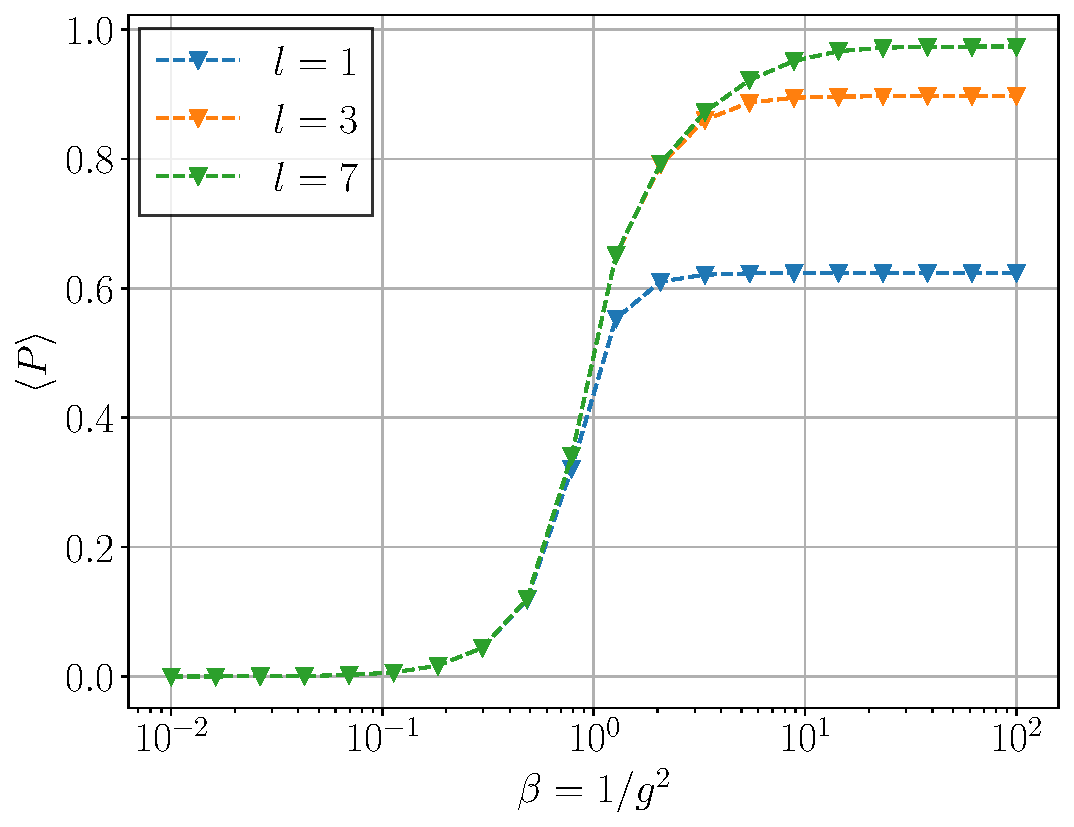
\includegraphics[width=0.7\textwidth]{../images/PlaquetteExp2x2PBC.pdf}};
  \node[above of=p, yshift=3cm] () {$\Braket{P} = \Braket{\sum_{\vec{r}}\frac{\hat{P}_{\vec{r}}+\hat{P}_{\vec{r}}^{\dag}}{2}}$, 
  $\hat{H}=\frac{g^2}{2}\sum_{\vec{r}}(\hat{E}_{\vec{r}, x}^2+\hat{E}_{\vec{r}, y}^2)-\frac{1}{2a^2g^2}\sum_{\vec{r}}(\hat{P}_{\vec{r}}+\hat{P}_{\vec{r}}^\dag)$};
\end{tikzpicture}

		\end{center}
		\caption{Plaquette Erwartungswerte für ein $2\times 2$ Gitter mit PBC.}\label{fig:2exp}
	\end{figure}
\end{frame}

\begin{frame}
	\begin{figure}[h]
		\begin{center}
			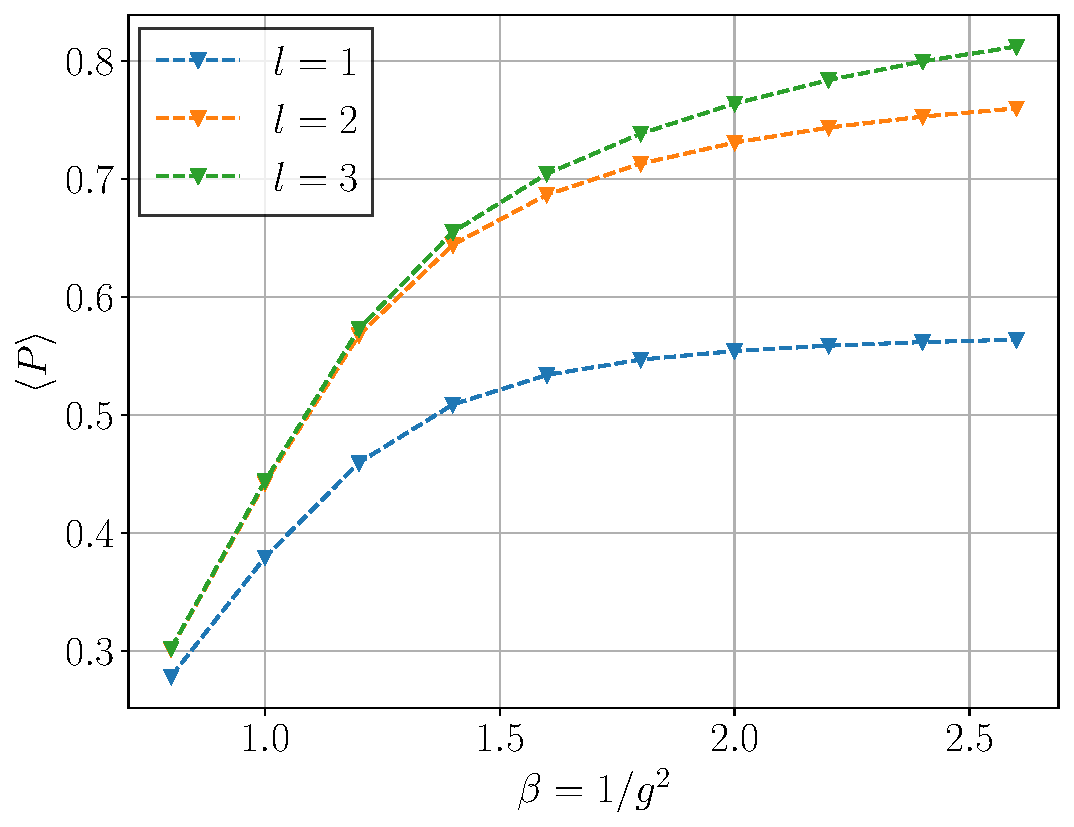
\includegraphics[width=0.8\textwidth]{images/PlaquetteExp3x3PBC.pdf}
		\end{center}
		\caption{Plaquette Erwartungswerte für ein $3\times 3$ Gitter mit PBC.}\label{fig:3exp}
	\end{figure}
\end{frame}

\section{Resultate: Quark-Antiquark Potential}
\begin{frame}
	\begin{columns}
		\begin{column}{0.3\textwidth}
			\begin{itemize}
				\item $V=\langle\hat{H}\rangle-\langle\hat{H}_0\rangle$
        \item $g=\num{1}, a=\num{1}$
				\item $3\times 3$
			\end{itemize}
			\scalebox{0.7}{
					\begin{tikzpicture}[thick,decoration={
					markings,
					mark=at position 0.5 with {\arrow{>}}}
		]

		\tikzset{
			site/.style={
					circle, draw=gray, fill=gray!20, line width=1.5pt, inner sep=0pt, outer sep=4pt, minimum size=0.4cm
				},
			pcharge/.style={
					circle, draw=red, fill=red!20, line width=1.5pt, inner sep=0pt, outer sep=4pt, minimum size=0.4cm
				},
			ncharge/.style={
					circle, draw=blue, fill=blue!20, line width=1.5pt, inner sep=0pt, outer sep=4pt, minimum size=0.4cm
				},
		}
    \node[](a1){};
		\node[pcharge, right of=a1, xshift=1cm](s1){\textbf{$+$}};
		\node[site, right=0.8cm of s1](s2){};
		\node[site, right=0.8cm of s2](s3){};
		\node[ncharge, above=0.8cm of s1](s4){\textbf{-}};
		\node[site, above=0.8cm of s2](s5){};
		\node[site, above=0.8cm of s3](s6){};
		\node[site, above=0.8cm of s4](s7){};
		\node[site, above=0.8cm of s5](s8){};
		\node[site, above=0.8cm of s6](s9){};

    \node[above of=s9, yshift=-0.4cm, xshift=-1.5cm](t1){Normal};


		\draw[postaction={decorate}] (s1)--(s2);
		\draw[postaction={decorate}] (s2)--(s3);

		\draw[postaction={decorate}] (s1)--(s4);
		\draw[postaction={decorate}] (s2)--(s5);
		\draw[postaction={decorate}] (s3)--(s6);

		\draw[postaction={decorate}] (s4)--(s5);
		\draw[postaction={decorate}] (s5)--(s6);

		\draw[postaction={decorate}] (s4)--(s7);
		\draw[postaction={decorate}] (s5)--(s8);
		\draw[postaction={decorate}] (s6)--(s9);

		\draw[postaction={decorate}] (s7)--(s8);
		\draw[postaction={decorate}] (s8)--(s9);

		\node[site, below of=s1, yshift=-4cm](w1){};

		\node[pcharge, right=0.8cm of w1](w2){\textbf{$+$}};
		\node[site, right=0.8cm of w2](w3){};
		\node[site, above=0.8cm of w1](w4){};
		\node[ncharge, above=0.8cm of w2](w5){\textbf{-}};
		\node[site, above=0.8cm of w3](w6){};
		\node[site, above=0.8cm of w4](w7){};
		\node[site, above=0.8cm of w5](w8){};
		\node[site, above=0.8cm of w6](w9){};


    \node[above of=w9, yshift=-0.4cm, xshift=-1.5cm](t2){Offset};


		\draw[postaction={decorate}] (w1)--(w2);
		\draw[postaction={decorate}] (w2)--(w3);

		\draw[postaction={decorate}] (w1)--(w4);
		\draw[postaction={decorate}] (w2)--(w5);
		\draw[postaction={decorate}] (w3)--(w6);

		\draw[postaction={decorate}] (w4)--(w5);
		\draw[postaction={decorate}] (w5)--(w6);

		\draw[postaction={decorate}] (w4)--(w7);
		\draw[postaction={decorate}] (w5)--(w8);
		\draw[postaction={decorate}] (w6)--(w9);

		\draw[postaction={decorate}] (w7)--(w8);
		\draw[postaction={decorate}] (w8)--(w9);

	\end{tikzpicture}


			}
		\end{column}
		\begin{column}{0.8\textwidth}
			\begin{figure}[h]
				\begin{center}
					Quark-Antiquark Potential
					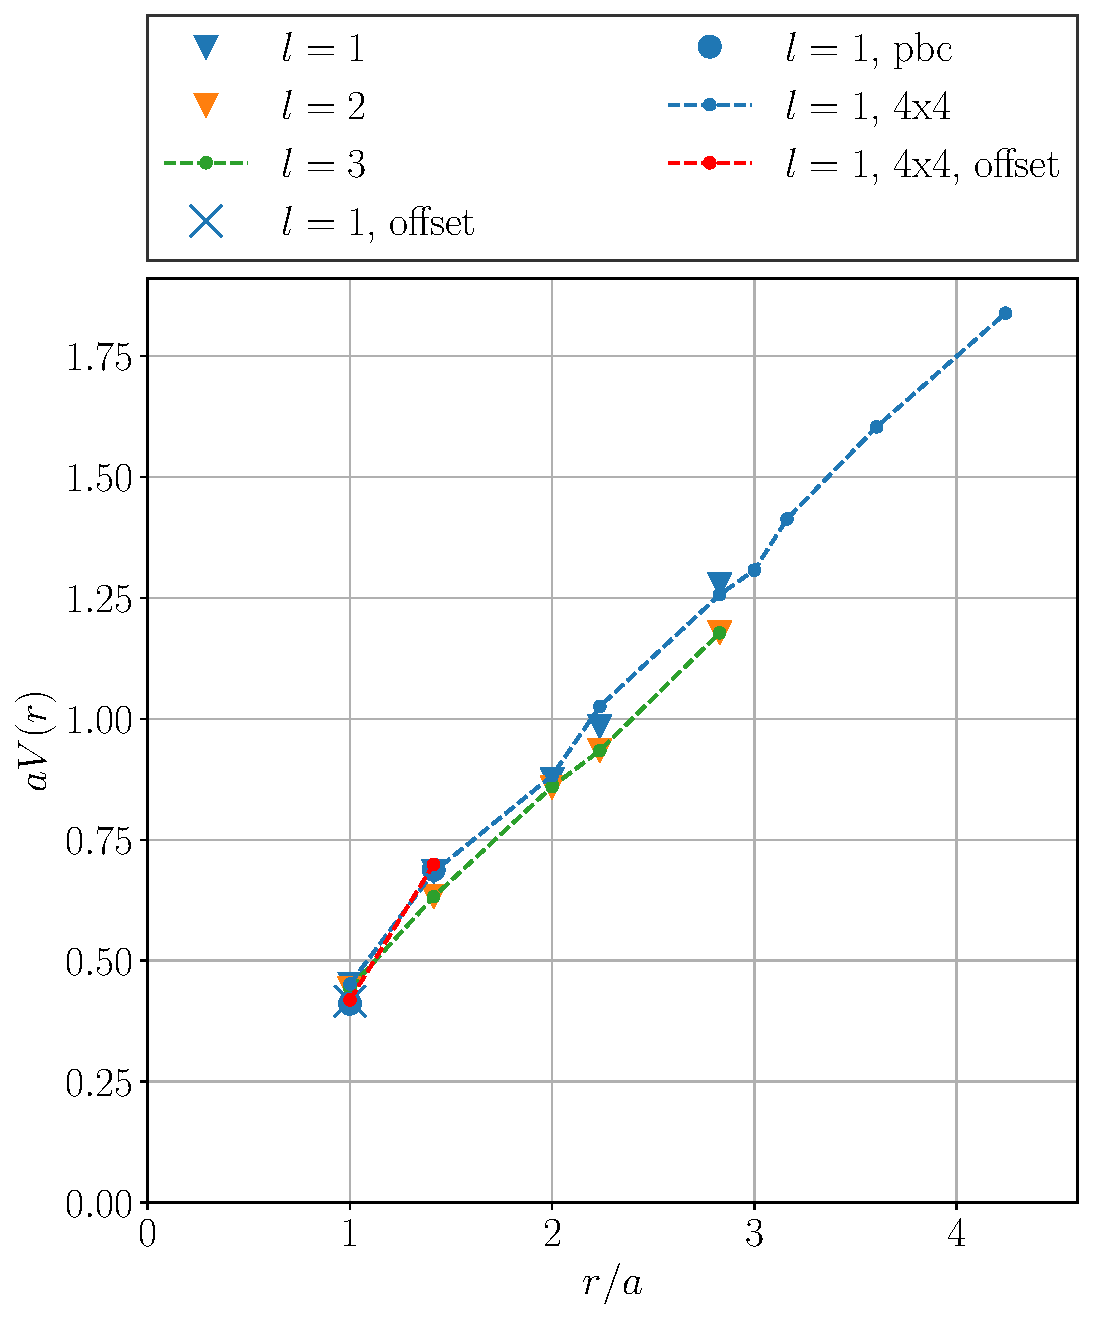
\includegraphics[width=0.7\textwidth]{images/quark_antiquark_potential_g_1.pdf}
				\end{center}
			\end{figure}
		\end{column}

	\end{columns}
\end{frame}

\begin{frame}
	\begin{columns}
		\begin{column}{0.5\textwidth}
      \hspace{80pt}$g=\num{5}$
			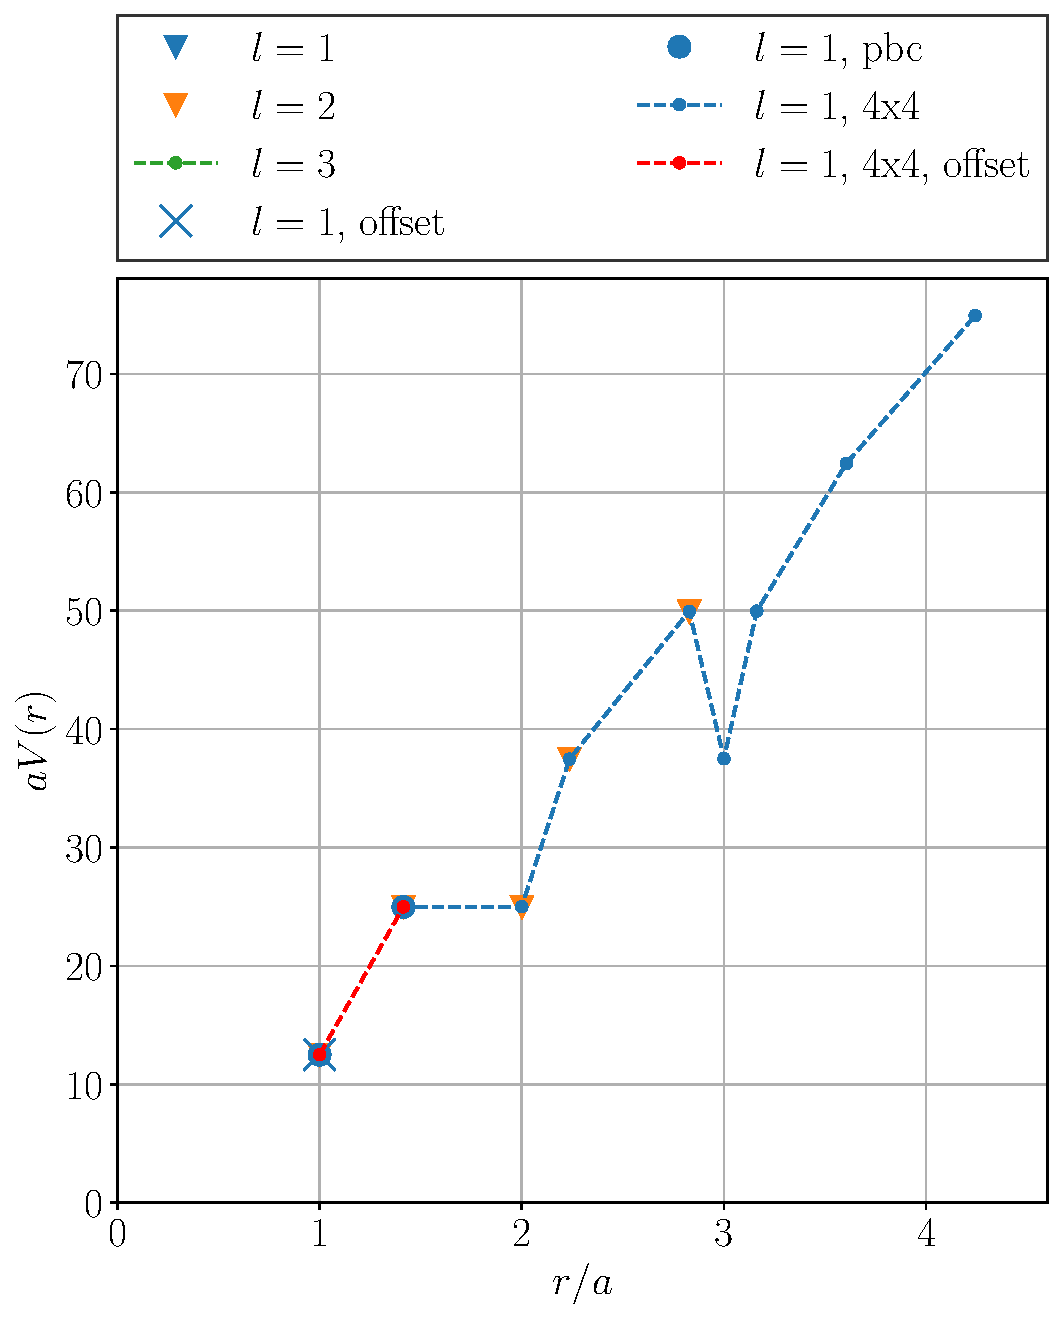
\includegraphics[width=1\textwidth]{images/quark_antiquark_potential_g_5.pdf}
		\end{column}
		\begin{column}{0.5\textwidth}
			\hspace{80pt}$g=\num{0.5}$
			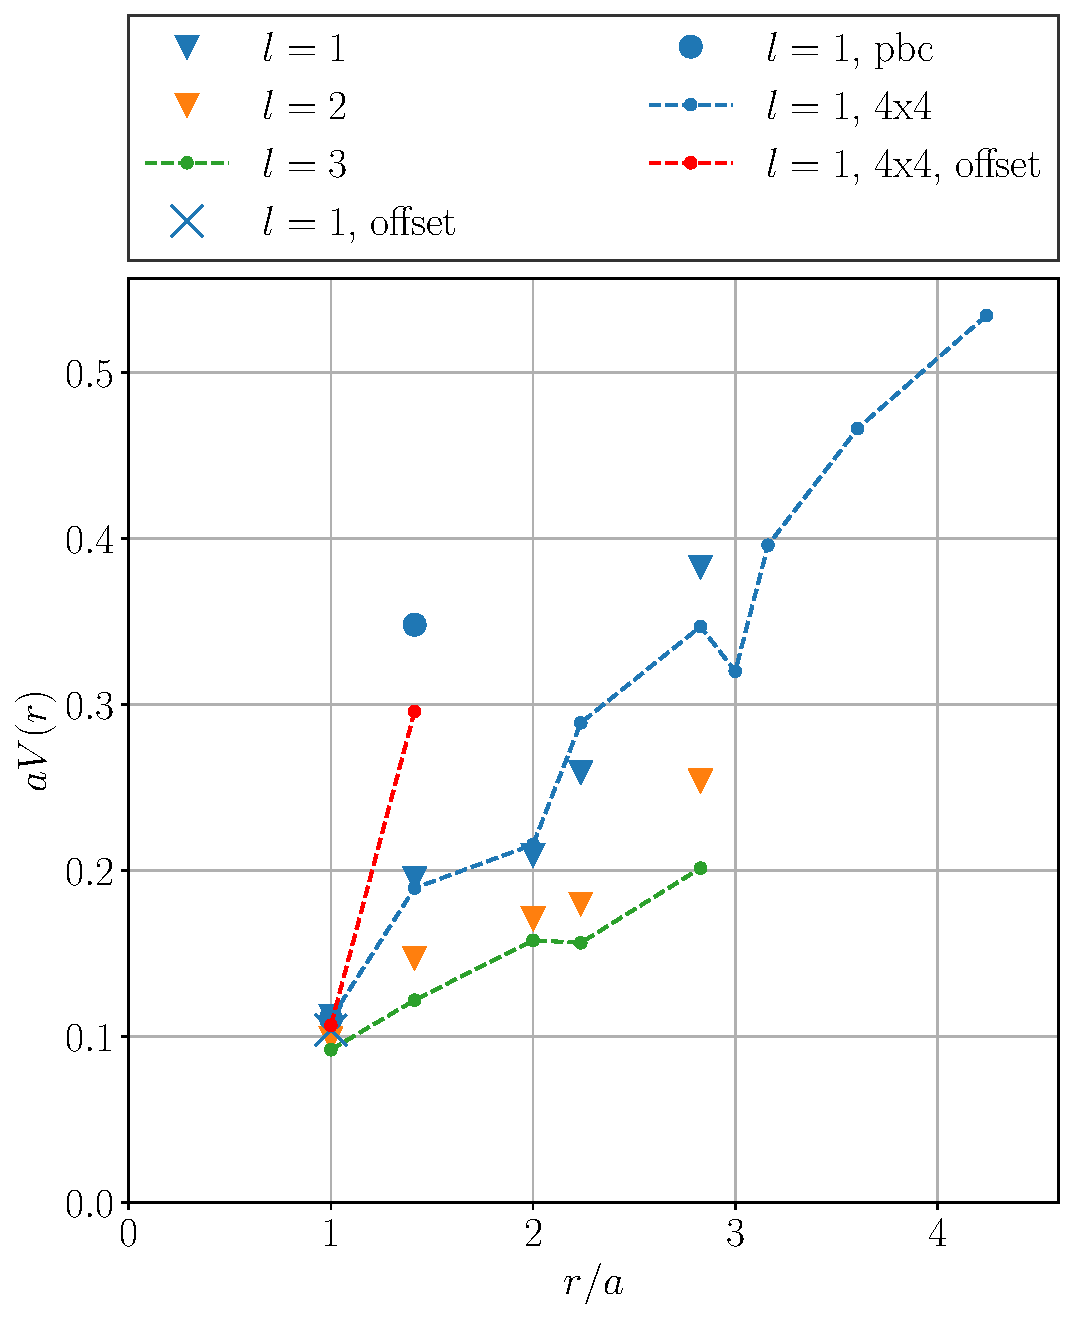
\includegraphics[width=1\textwidth]{images/quark_antiquark_potential_g_0.5.pdf}
		\end{column}

	\end{columns}
\end{frame}

\begin{frame}
	\begin{columns}
		\begin{column}{0.3\textwidth}
		\end{column}
		\begin{column}{0.8\textwidth}
			\hspace{80pt}$g=\num{0.1}$
			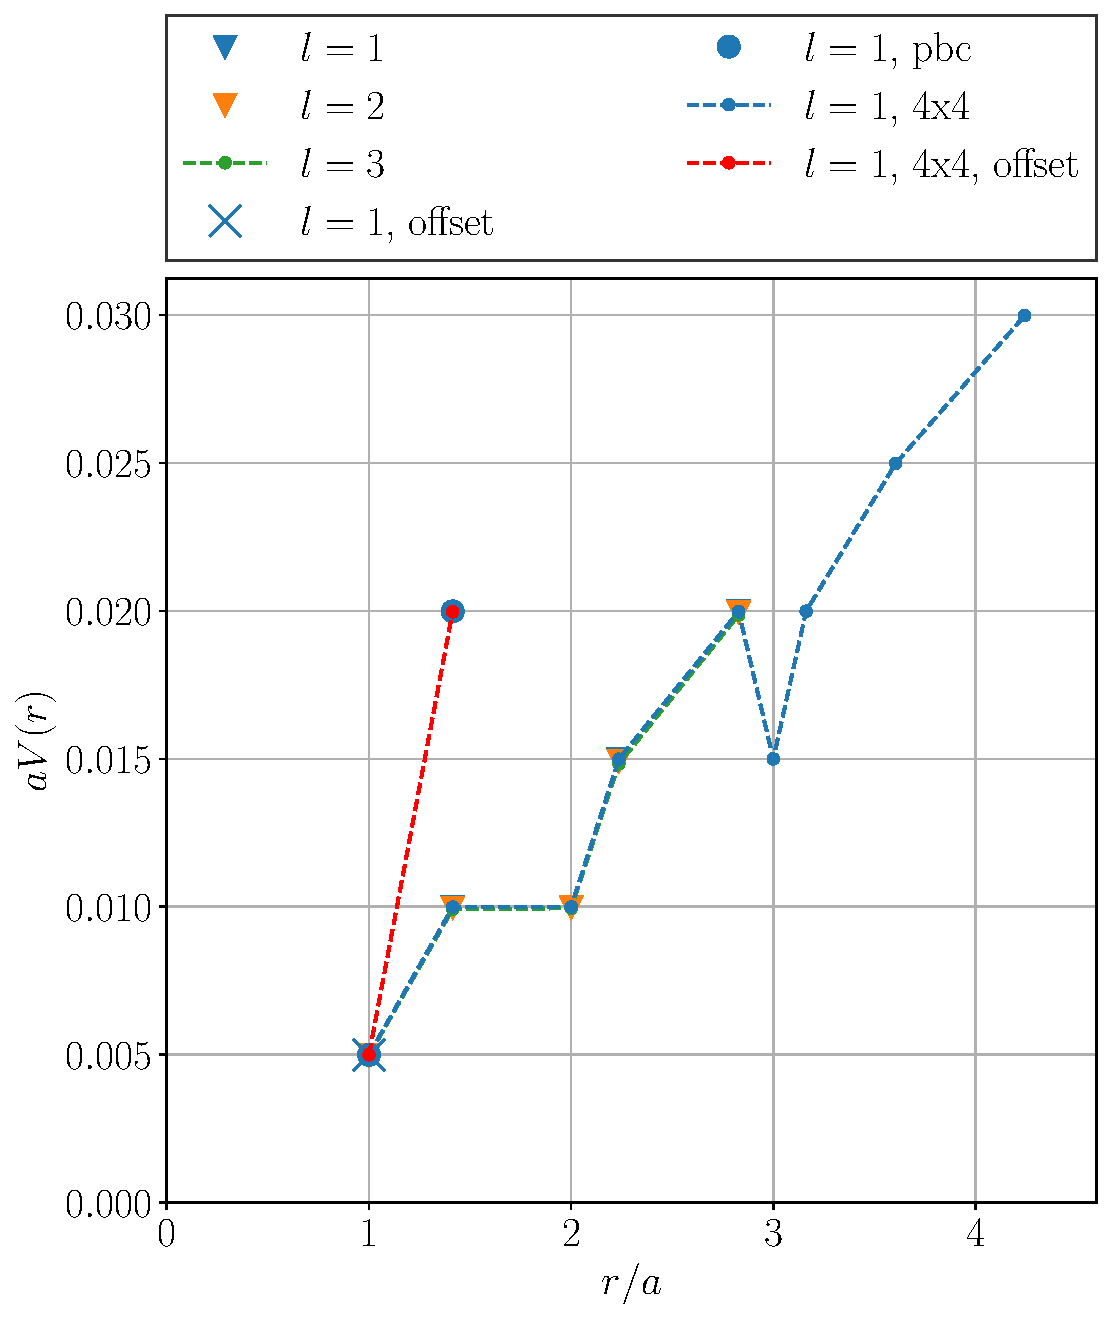
\includegraphics[width=0.7\textwidth]{images/quark_antiquark_potential_g_0.1.pdf}
		\end{column}

	\end{columns}
\end{frame}

\section{Outlook}
\begin{frame}
	\frametitle{Outlook}
	\begin{itemize}
		\item VQE / Tensor Netzwerke
		\item Größere Gitter
		\item running coupling mit step scaling
		\item Einheiten / Gitterabstand bestimmen
		      \begin{itemize}
			      \item schwer, da (2+1) Dimensional
		      \end{itemize}
		\item (3+1) Dimensional
		\item an realen Werten kallibrieren und schwer messbare Potentiale ermitteln
    \item SU(2), SU(3)
	\end{itemize}
\end{frame}

\begin{frame}
	\frametitle{Outlook}
	\begin{figure}[h]
		\center\input{tikz/outlook.tex}
	\end{figure}
\end{frame}

\section{Abschluss}
\begin{frame}
	\,\\
   \huge{\hspace{105pt}Vielen Dank für\\ \hspace{85pt}eure Aufmerksamkeit}

\end{frame}

\end{document}

